\documentclass[xcolor=svgnames,aspectratio=169]{beamer}
\usetheme{Boadilla}

\usepackage[utf8]{inputenc}
\usepackage[T1]{fontenc}
\usepackage{lmodern}
\usepackage{sourcecodepro}
\usepackage[whole]{bxcjkjatype}

\usepackage[backend=biber,style=numeric-comp,sorting=none]{biblatex}
\addbibresource{slides.bib}
\setbeamertemplate{bibliography item}{\insertbiblabel}

\usepackage{listings}
\lstset{
  language=Octave,
  keywordstyle=\color{blue},
  showstringspaces=false,
  stringstyle=\color{magenta},
  commentstyle=\color{DarkGreen},
}
\usepackage{textcomp}
\usepackage{tikz}
\usetikzlibrary{tikzmark,overlay-beamer-styles,babel}

\usepackage{mathtools}
\usepackage{multimedia}
\usepackage{siunitx}
\usepackage{pifont}
\usepackage{tikz}
\newcommand*\colorcheck[1]{%
  \expandafter\newcommand\csname #1check\endcsname{\textcolor{#1}{\ding{52}}}%
}
\colorcheck{green}
\usepackage{microtype}
\DisableLigatures{encoding = OT1}
\def\UrlFont{\fontencoding{OT1}\selectfont}

\title[APA - Arbitrary Precision Arithmetic toolbox]{APA - An Arbitrary Precision Arithmetic toolbox}
\subtitle{for Octave and Matlab}
\author[Kai T. Ohlhus]{
  オールフス カイトーベン \\
  OHLHUS, Kai Torben}
\institute[TWCU]{
  Graduate School of Science \\
  Tokyo Woman's Christian University}
\date[November 27, 2021]{
"Development of Verified Numerical Computations for Mathematical Modeling" \\
JST/CREST Result Briefing
{\footnotesize\url{http://verifiedby.me/nvr2021/}} \\
(online) \\[1em]
November 27, 2021}
\titlegraphic{
\hfill\includegraphics[height=1em]{res/images/cc-by-sa}
}


\begin{document}

{
\usebackgroundtemplate{
  \vbox to \paperheight{\vfil\hbox to \paperwidth{\hfil
  \tikz\node[opacity=0.15] {
  %\includegraphics[width=0.6\paperwidth]{res/images/logo}
  };
  \hfil}\vfil}
}
\frame{\titlepage}
}


\section{Why yet another toolbox?}
\frame{\tableofcontents}
\begin{frame}{Family of free GNU Multiple Precision Libraries}

\begin{itemize}\itemsep0.5em

\item
\textbf{GMP - GNU Mult. Prec. Arithmetic Library}\footnote{\tiny
\url{https://gmplib.org/}}
(C/C++, version 6.2.1; since 1991)
\begin{itemize}
\item
supports: signed integers, rational numbers, and floating-point numbers

\item
arithmetic and logic functions for supported data types

\item
focus: \textbf{speed, cryptography}
\end{itemize}

\item
\textbf{MPFR - GNU Mult. Prec. Fl.-Point Reliable Library}\footnote{\tiny
\url{https://www.mpfr.org/}}
(C, version 4.1.0; since 2000)
\begin{itemize}
\item
supports: floating-point numbers (arithmetic and logic functions)

\item
focus: \textbf{correct rounding}, precise semantics (IEEE 754)
\end{itemize}

\item
\textbf{MPC - GNU Mult. Prec. Complex Library}\footnote{\tiny
\url{http://www.multiprecision.org/}}
(C, version 1.2.1; since 2003)
\begin{itemize}
\item
addition: \textbf{complex} floating-point numbers
\end{itemize}

\bigskip

\item
Many interfaces (C++, Python, ...) are available.

\end{itemize}

\end{frame}



\begin{frame}{Comparable Matlab/Octave toolboxes}

\begin{itemize}\itemsep0.5em

\item
\textbf{Matlab VPA (Variable-precision arithmetic,
Symbolic toolbox)}\footnote{\tiny
\url{https://www.mathworks.com/help/symbolic/vpa.html}}
\begin{itemize}
\item
Slow for dimensions > 200.
\end{itemize}

% Pavel Holoborodko (Yokohama, Japan)
\item
\textbf{Advanpix}\footnote{\tiny
\url{https://www.advanpix.com/}}
(version 4.8.5.14569; since 2010)
{\color{red} Very fast and complete!}
\begin{itemize}
\item
{\color{blue} closed source} (P-code), proprietary license

\item
Matlab only
\end{itemize}

% Jean-Daniel Bancal (Switzerland)
\item
\textbf{GEM - Gmp Eigen Matrix Library}\footnote{\tiny
\url{https://gem-library.github.io/}}
(version 2.0.2; since 2016)
\begin{itemize}
\item
free, open source (MPL-2.0, others)

\item
Matlab and Octave
\end{itemize}

% Ben Barrowes (USA)
\item
\textbf{mptoolbox}\footnote{\tiny
\url{https://sourceforge.net/projects/mptoolbox/}
and
\url{https://www.mathworks.com/matlabcentral/fileexchange/6446-multiple-precision-toolbox-for-matlab}}
(version 1.5; since 2004)
\begin{itemize}
\item
free, open source (BSD-3-Clause)

\item
Matlab and "Octave" (needs some adaptions)
\end{itemize}

\end{itemize}

\end{frame}


\section{APA toolbox}
\frame{\tableofcontents[currentsection]}
\begin{frame}{What makes APA different?}
\framesubtitle{A real wrapper around the plain C functions.}


\end{frame}


\begin{frame}[fragile]{What makes APA different?}
\framesubtitle{Almost drop-in compatible with C Code\footnote{Example
from https://www.mpfr.org/sample.html (2021-11-19).}.}

\begin{columns}
\begin{column}[T]{0.3\textwidth}
\includegraphics[width=\linewidth]{res/images/mpfr_example}
\end{column}
\begin{column}[T]{0.5\textwidth}
APA {\color{blue}Low-Level} interface (control, "speed"): \\[1em]

\begin{lstlisting}[basicstyle=\tiny]
t = mpfr_t (1.0, 200, MPFR_RNDD);
s = mpfr_t (1.0, 200, MPFR_RNDD);
u = mpfr_t (nan, 200);

for i = 1:100
  mpfr_mul_ui (t, t, i, MPFR_RNDU);
  mpfr_set_d (u, 1.0, MPFR_RNDD);
  mpfr_div (u, u, t, MPFR_RNDD);
  mpfr_add (s, s, u, MPFR_RNDD);
end

fprintf ('Sum is ');
disp (s, MPFR_RNDD);
\end{lstlisting}
\end{column}
\end{columns}

\end{frame}


\begin{frame}[fragile]{What makes APA different?}
\framesubtitle{Almost drop-in compatible with C Code\footnote{Example
from https://www.mpfr.org/sample.html (2021-11-19).}.}

\begin{columns}
\begin{column}[T]{0.3\textwidth}
\includegraphics[width=\linewidth]{res/images/mpfr_example}
\end{column}
\begin{column}[T]{0.5\textwidth}
APA {\color{blue}High-Level} interface (convenience): \\[1em]

\begin{lstlisting}[basicstyle=\tiny]
% Setup default values
setround = @(rnd) ...
mpfr_set_default_rounding_mode (rnd);
mpfr_set_default_prec (200);

setround (MPFR_RNDD)
t = mpfr_t (1.0);
s = mpfr_t (1.0);

for i = 1:100
  setround (MPFR_RNDU);
  t = t * i;
  setround (MPFR_RNDD);
  s = s + (1 / t);
end

fprintf ('Sum is ');
disp (s);
\end{lstlisting}
\end{column}
\end{columns}

\end{frame}



\section{Benchmark}
\frame{\tableofcontents[currentsection]}
\begin{frame}{Benchmark (1/4)}

\begin{itemize}\itemsep1em
\item
Test system:
\begin{itemize}
\item
Intel(R) Xeon(R) Platinum 8276 CPU @ 2.20GHz,
28 cores (56 threads),
1 TB RAM

\item
Matlab R2021a (Update 5) on CentOS 7 \\[0.5em]

\item
{\color{blue}
APA (1.0.0), Advanpix (4.8.5.14569), GEM (2.0.2), VPA (R2021a)}
\end{itemize}

\item
Tests with \lstinline|A = rand(N,N)| and \lstinline|b = A * ones(N,1)|:

\begin{itemize}
\item
Matrix-Matrix-Multiplication
$\quad$
\lstinline|A * A|

\item
LU-factorization
$\qquad\qquad\qquad$
\lstinline|[L,U] = lu (A)|

\item
Solve $Ax = b$
$\qquad\qquad\qquad\quad\;$
\lstinline|x = A \\ b|\\[0.5em]

\item
Precisions \cite[Chapter 3.1]{Muller2018}:

\begin{tabular}{|c|c|c|}
\hline
Name & Binary & Decimal\footnote{\scriptsize decimal precision
:= $\lfloor \text{binary precision} \times \log_{10}(2) \rfloor$,
see "bits2digits" in \url{http://www.holoborodko.com/pavel/mpfr/}.} \\
\hline\hline
"double"    &  53 & 15 \\
"quadruple" & 113 & 34 \\
"octuple"   & 237 & 71 \\
\hline
\end{tabular}

\end{itemize}

\end{itemize}

\end{frame}


\begin{frame}{Benchmark (2/4)}

\begin{columns}
\begin{column}{0.3\textwidth}
\begin{figure}
\centering
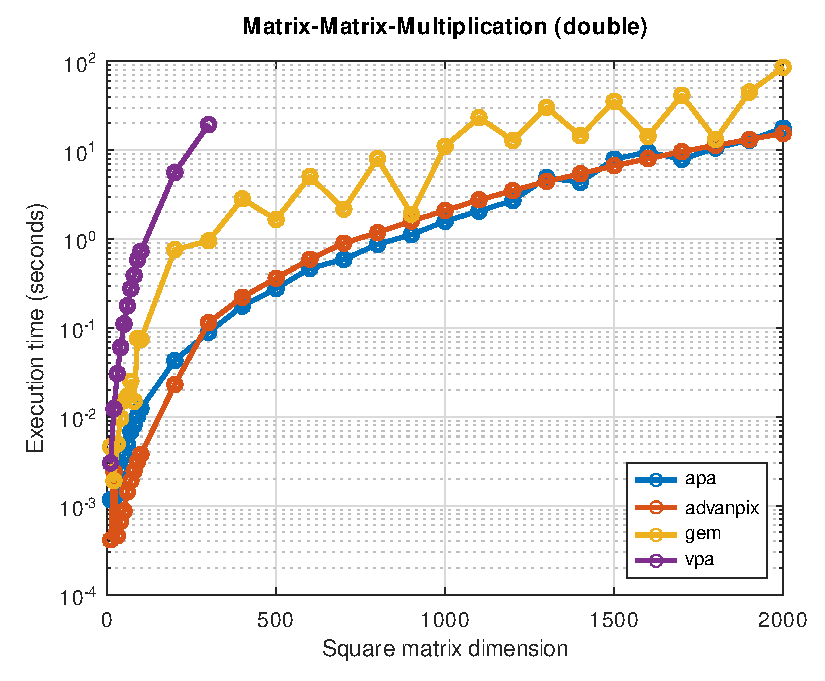
\includegraphics[width=1.0\linewidth]{res/data/2021-11-24_run-01-mmm-double-semilogy}
\end{figure}
\end{column}
\begin{column}{0.3\textwidth}
\begin{figure}
\centering
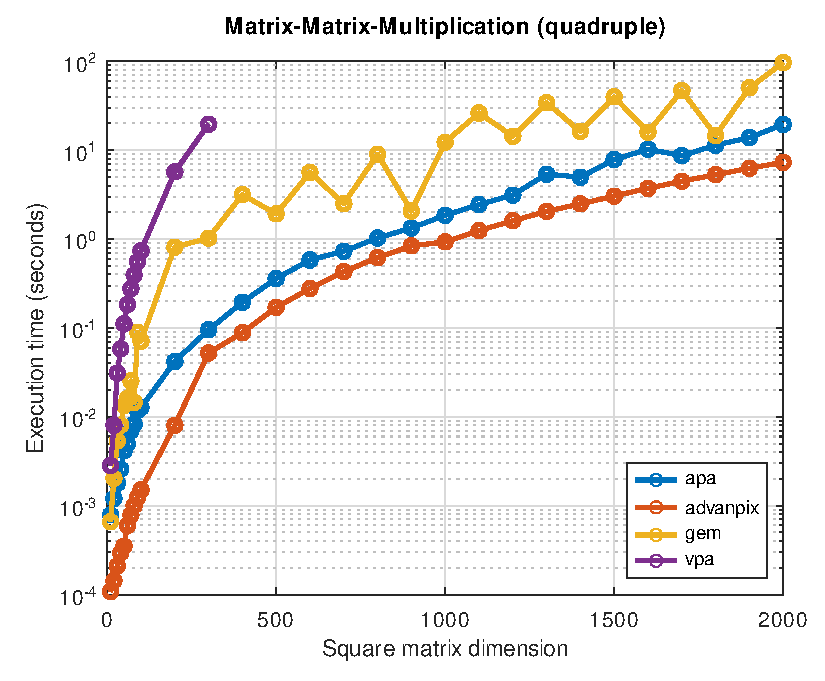
\includegraphics[width=1.0\linewidth]{res/data/2021-11-24_run-01-mmm-quadruple-semilogy}
\end{figure}
\end{column}
\begin{column}{0.3\textwidth}
\begin{figure}
\centering
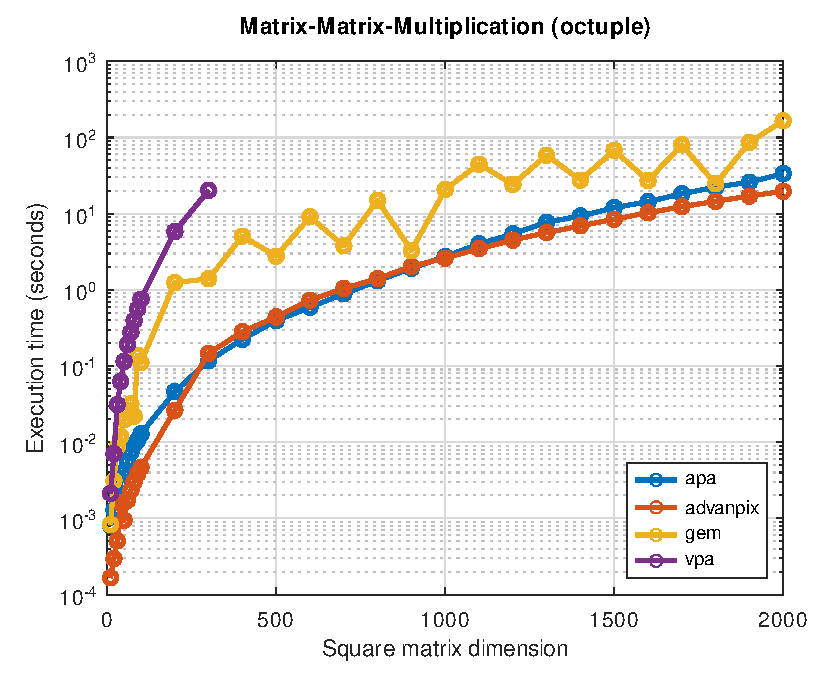
\includegraphics[width=1.0\linewidth]{res/data/2021-11-24_run-01-mmm-octuple-semilogy}
\end{figure}
\end{column}
\end{columns}

\end{frame}


\begin{frame}{Benchmark (3/4)}

\begin{columns}
\begin{column}{0.3\textwidth}
\begin{figure}
\centering
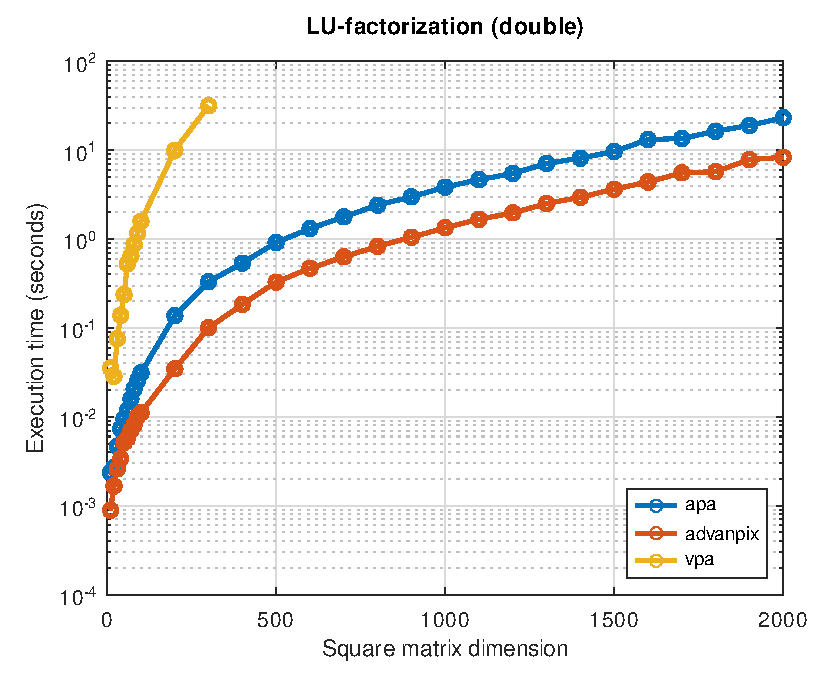
\includegraphics[width=1.0\linewidth]{res/data/2021-11-24_run-01-lu-double-semilogy}
\end{figure}
\end{column}
\begin{column}{0.3\textwidth}
\begin{figure}
\centering
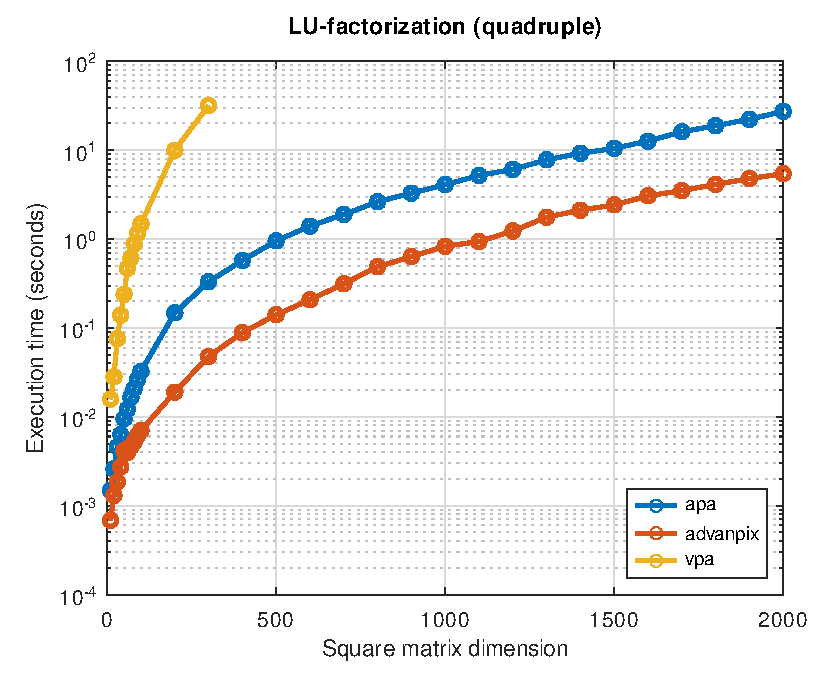
\includegraphics[width=1.0\linewidth]{res/data/2021-11-24_run-01-lu-quadruple-semilogy}
\end{figure}
\end{column}
\begin{column}{0.3\textwidth}
\begin{figure}
\centering
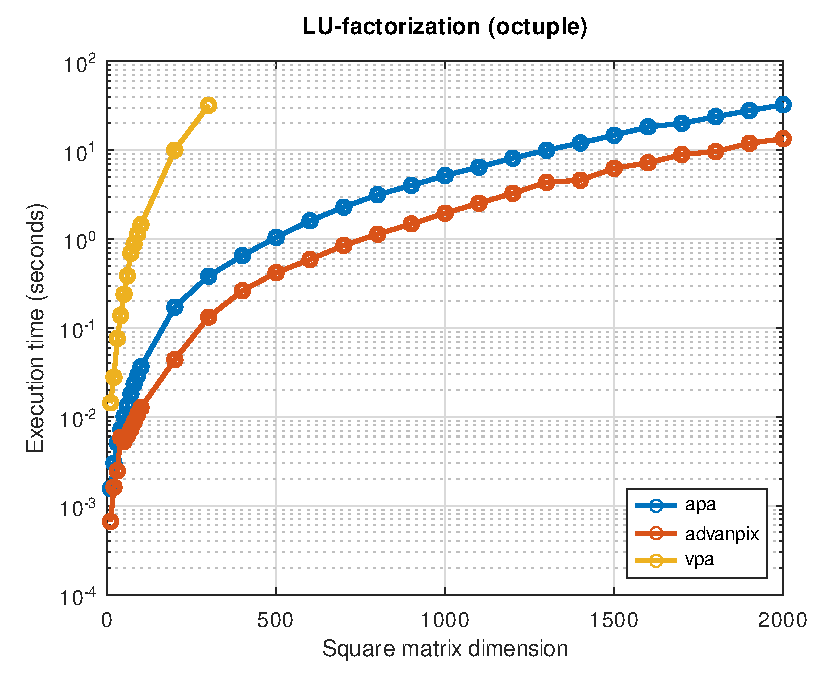
\includegraphics[width=1.0\linewidth]{res/data/2021-11-24_run-01-lu-octuple-semilogy}
\end{figure}
\end{column}
\end{columns}

\end{frame}


\begin{frame}{Benchmark (4/4)}

\begin{columns}
\begin{column}{0.3\textwidth}
\begin{figure}
\centering
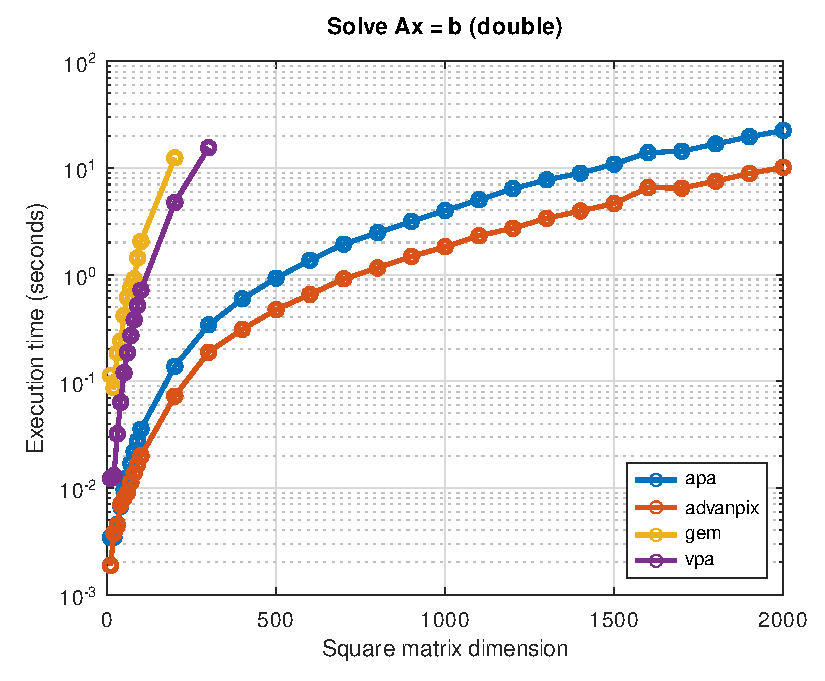
\includegraphics[width=1.0\linewidth]{res/data/2021-11-24_run-01-lin-double-semilogy}
\end{figure}
\end{column}
\begin{column}{0.3\textwidth}
\begin{figure}
\centering
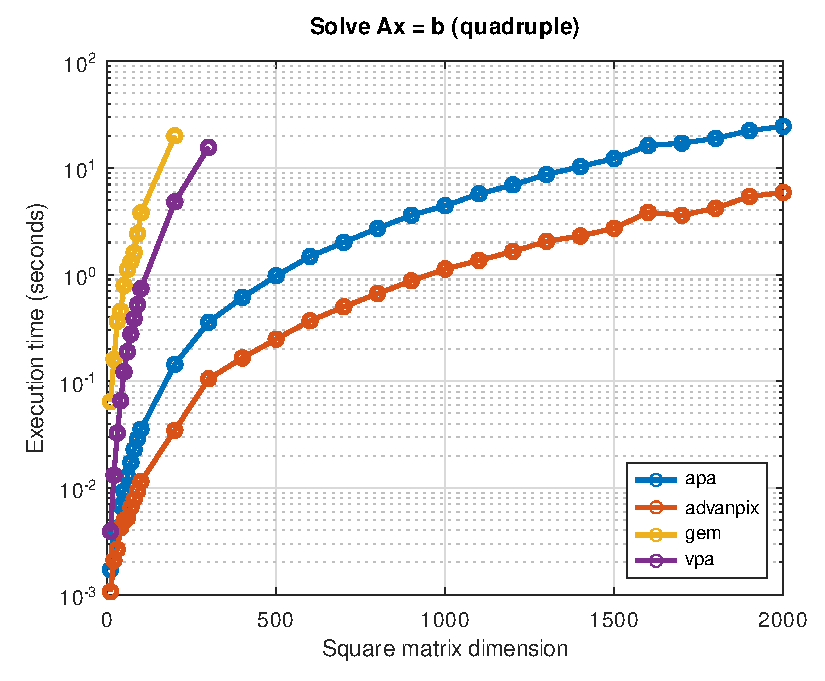
\includegraphics[width=1.0\linewidth]{res/data/2021-11-24_run-01-lin-quadruple-semilogy}
\end{figure}
\end{column}
\begin{column}{0.3\textwidth}
\begin{figure}
\centering
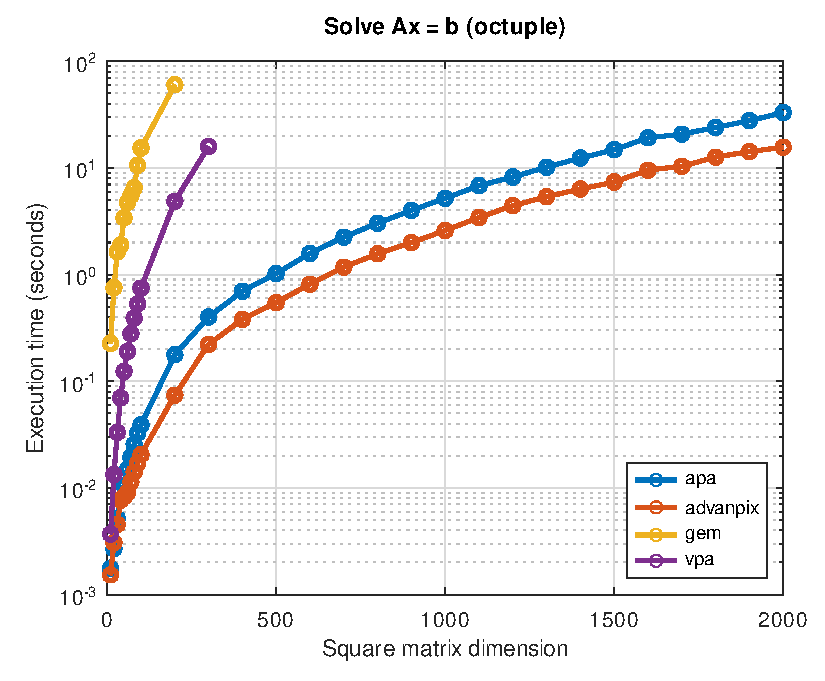
\includegraphics[width=1.0\linewidth]{res/data/2021-11-24_run-01-lin-octuple-semilogy}
\end{figure}
\end{column}
\end{columns}

\end{frame}



\section{Summary}
\frame{\tableofcontents[currentsection]}
\begin{frame}{Summary and outlook}

APA is an arbitrary precision arithmetic toolbox for Octave/Matlab:

\begin{itemize}\itemsep0.5em
\item
\textbf{Free, extensible, and fast} compared to other toolboxes.

\item
\textbf{Very easy installation} from inside Octave/Matlab command window.

\item
Microsoft Windows, macOS, and Linux support.
\end{itemize}

\bigskip

What comes next?
\begin{itemize}\itemsep0.5em
\item
Extend implementation:
\begin{itemize}
\item
Cholesky factorization, SVD-, Eigenvalue-decomposition

\item
MPC interface (complex data)

\item
Sparse and N-dimensional data type and algorithms

\item
Research and test published MPFR-algorithms
(dot-product \cite{Isupov2020}, matrix multiplication \cite{Kouya2016}, ...)

\item
Usage of other MPFR-based libraries (MPLAPACK \cite{Nakata2021}, ...)?
\end{itemize}

\item
Use MPFR ternary return value to detect accuracy loss in algorithms.
\end{itemize}
\end{frame}


\begin{frame}
\begin{center}
\textbf{\Large Thank you for your attention!}

\bigskip

\bigskip

\textbf{\Large Questions?}
\vfill\footnotesize
Slides and sources available at:
{\color{DarkBlue}\url{https://github.com/siko1056/slides_nvr2021}} \\[1em]
$\qquad\qquad\quad\;\;$APA-Toolbox:
{\color{DarkBlue}\url{https://github.com/gnu-octave/pkg-apa}}

\end{center}
\end{frame}



% Backup slides.
\newcounter{finalframe}
\setcounter{finalframe}{\value{framenumber}}



\section*{References}



\begin{frame}[allowframebreaks,noframenumbering]
\frametitle{References}
\printbibliography
\end{frame}



\setcounter{framenumber}{\value{finalframe}}

\end{document}
